\documentclass[a4paper,11pt,titlepage]{article}

\usepackage{latexsym}
\usepackage{graphicx}
\usepackage{float}
\usepackage{url}
\usepackage{unicode}
\usepackage[polish]{babel}
\usepackage{titlesec}
\usepackage{listings}
\usepackage{xcolor}
\usepackage{setspace}
\usepackage{subfig}
\usepackage{tabularx}
\usepackage{courier}
\DeclareUnicodeCharacter{200B}{{\hskip 0pt}}

\definecolor{codeblue}{rgb}{0,0,0.6}
\definecolor{codegray}{rgb}{0.5,0.5,0.5}
\definecolor{codepurple}{rgb}{0.58,0,0.82}
\definecolor{backcolour}{rgb}{0.96,0.96,0.96}

\lstdefinestyle{code}{
    backgroundcolor=\color{backcolour},
    keywordstyle=\color{codeblue},
    numberstyle=\tiny\color{codegray},
    stringstyle=\color{codeblue},
    basicstyle=\ttfamily\footnotesize,
    breakatwhitespace=false,
    breaklines=true,
    captionpos=b,
    keepspaces=true,
    numbers=left,
    numbersep=3pt,
    showspaces=false,
    showstringspaces=false,
    showtabs=false,
    tabsize=1,
    basicstyle=\small
}

\lstset{style=code}

\newcommand{\sectionbreak}{\clearpage}
\author{Adam Talarczyk}
\title{Symulacje Monte Carlo}
\frenchspacing
\begin{document}
\begin{titlepage}
    \begin{center}

        \Huge
        \textbf{WYDZIAŁ NAUK ŚCISŁYCH I TECHNICZNYCH}
        
        
        \vspace{1.5cm}
	   Symulacje Komputerowe
        \LARGE
        
	\vspace{2cm}
	
	Sprawozdanie ``Symulacja zdarzeń dyskretnych''

	\vspace{1cm}
	Adam Talarczyk, Mateusz Wrzoł
	
	\vspace{5cm}
        \vfill

        \vspace{0.8cm}
	\Large
        Uniwersytet Śląski, Sosnowiec, 2021

    \end{center}
\end{titlepage}
\newpage

%\tableofcontents
% \newpage


\section{Zadanie 1}
Wykonać symulację bramek autostradowych uwzględniając następujące założenia:
\begin{itemize}
	\item Dostępne są cztery bramki. Na trzech bramkach kierowcy mogą płacić kartą i gotówką. Na jednej bramce kierowcy mogą płacić tylko kartą.
	\item Czas trwania obsługi na bramce w przypadku płatności gotówką jest opisany rozkładem normalnym o średniej M1 minuty i odchyleniu standardowym SD1 minuty.
	\item Czas trwania obsługi na bramce w przypadku płatności kartą jest opisany rozkładem normalnym o średniej M2 minuty i odchyleniu standardowym SD2 minuty.
	\item Odstęp czasu pomiędzy nadjeżdżającymi samochodami jest opisany rozkładem wykładniczym o parametrze lambda = L (wartość oczekiwana wynosi 1/L minuty, L odpowiada średniej liczbie pojazdów na minutę).
	\item Połowa kierowców zamierza dokonać płatności kartą a druga połowa gotówką. Nadjeżdżający kierowcy wybierają dostępną bramkę z najkrótszą kolejką. Płacący gotówką mają do wyboru 3 bramki. Płacący kartą wybierają spośród 4 bramek.
	Wartości parametrów
	\end{itemize}

\begin{figure}[H]
 \centering
 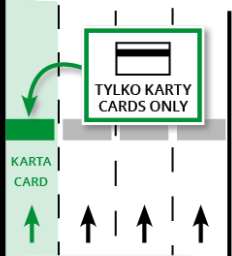
\includegraphics[width=0.35\columnwidth]{img/tresc.PNG}
 \caption{Wizualizacja}
 \label{fig:wykres1}
\end{figure}

Wartości parametrów SD1, SD2, M1 i M2 należy przyjąć według własnego uznania.

Wyznaczyć symulacyjnie zależność pomiędzy średnią liczbą pojazdów na minutę (L) i średnim czasem oczekiwania na przejazd przez bramki. Przedstawić tę zależność na wykresie.

W sprawozdaniu należy zamieścić treść zadania, kod źródłowy rozwiązania z opisem, wyniki symulacji i wykres.


% \ref{fig:wykres1}.

% \begin{figure}[H]
% \centering
% \includegraphics[width=1\columnwidth]{img/zad1.PNG}
% \caption{Przykład wykresu}
% \label{fig:wykres1}
% \end{figure}

\subsection{Rozwiązanie}


% \begin{table}[h!]
% \centering
% \begin{tabular}{ |c|c|c| } 
% \hline
% Próbka & Średnie przybliżenie $\pi$ & Błąd aproksymacji \\
% \hline
% 1	& 3,6 &	0,45840735 \\
% 10	& 3,04 &	0,10159265 \\
% \hline
%\end{tabular}
%\caption{Tablica z wynikami uzyskanymi w symulacji}
%\label{tab:res}
% \end{table}


\subsection{Kod źródłowy}

% \lstinputlisting[language=R, caption=opis, label={listing-label}]{../path/to/code.R}

\end{document}
